
\subsection{Análisis de Algoritmos de Ordenamiento}

Los cuatro algoritmos de ordenamiento muestran, en general, un crecimiento esperado para su complejidad teórica de \textbf{$O(n \log n)$}. Si miramos los tiempos de MergeSort, QuickSort y \texttt{std::sort} crecen de manera practicamnete paralela entre los cuatro tamaños evaluados ($n=10, 10^3, 10^5, 10^7$), ya que los cuatro comparten el mismo orden asintótico. En la práctica, Quick Sort y \texttt{std::sort} son los más rápidos. La razón es que ambos ordenan los datos ahí mismo (\textit{in-place}), ahorrándose el trabajo extra de pedir memoria y mover datos hacia estructuras auxiliares, cosa que Merge Sort sí tiene que hacer obligatoriamente.

\begin{figure}[H]
    \centering
    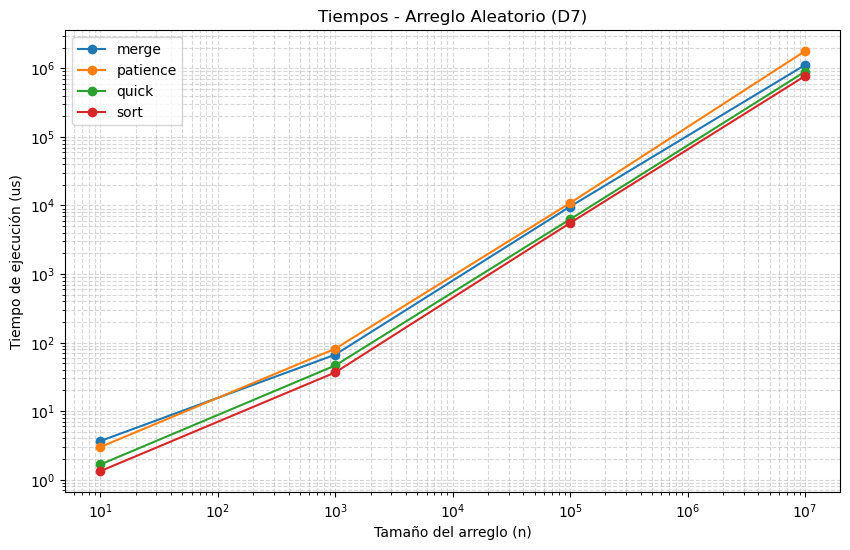
\includegraphics[width=0.7\linewidth]{sections/tiempos_aleatorio_D7.png}
    \caption{Tiempo de ejecución para arreglos aleatorios (Dominio D7).}
    \label{fig:sort_aleatorio_tiempo}
\end{figure}

El caso de Patience Sort es el más interesante de todos, porque su tiempo de ejecución no depende solo de la cantidad de datos ($n$), sino de qué tan desordenados vienen. Por ejemplo, en el dominio D7, para $n=10^7$, tarda cerca de 1.5 segundos (aproximadamente 1543796 us) en el caso ascendente, pero solo del orden de cientos de milisegundos en el caso descendente, una diferencia que no se observa en ningún otro algoritmo. 
Lo podemos explicar por como va el algoritmo funcionando internamente por que este va armando pilas como si fueran cartas de un solitario, si el arreglo viene de menor a mayor, como cada número es más grande que el anterior tiene que crear una pila completamente nueva por cada elemento (haciendo $n$ pilas en total, su peor caso). En cambio, si viene de mayor a menor, todos los elementos caben perfectamente uno sobre otro en una sola pila.  Como la complejidad real de Patience Sort es $O(n \log k)$, con $k$ el número de pilas resultante, y no simplemente $O(n \log n)$, este experimento demuestra de forma muy clara la diferencia entre la teoría general y el comportamiento del algoritmo según cómo vengan los datos de entrada.

En cuanto al uso de memoria, QuickSort es consistentemente el más eficiente, coherente con ser el único que ordena completamente \textit{in-place}. Patience Sort es el que más recursos consume: al mantener muchas pilas separadas usando arreglos bidimensionales (\verb|vector<vector<int>>|), gasta muchísima más memoria y tiempo de asignación que si usara un solo arreglo largo y continuo, además de requerir un \textit{heap} extra. MergeSort también supera a QuickSort por la reserva del arreglo auxiliar de tamaño $n$ que usa para la mezcla.

\begin{figure}[H]
    \centering
    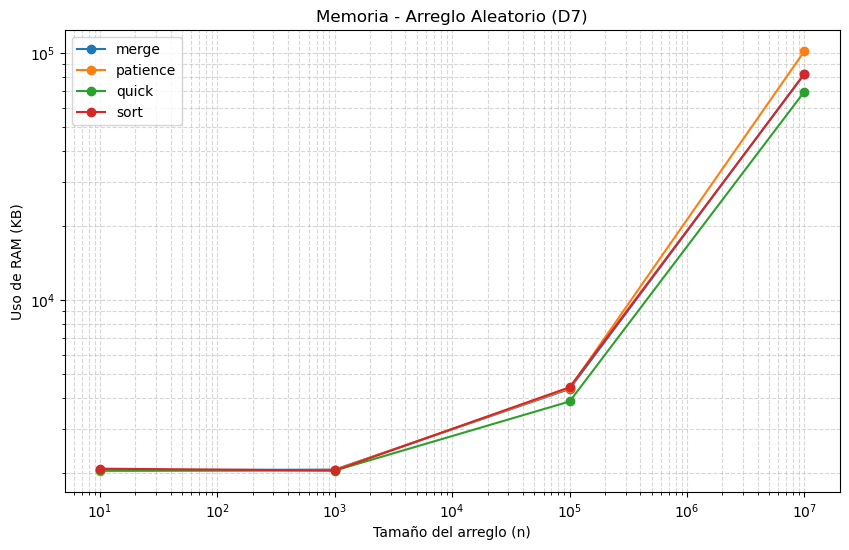
\includegraphics[width=0.7\linewidth]{sections/memoria_aleatorio_D7.png}
    \caption{Tiempo de ejecución para arreglos aleatorios (Dominio D7).}
    \label{fig:sort_aleatorio_mem}
\end{figure}

Un caso particular es \texttt{std::sort}: pese a ser \textit{in-place}, su consumo de memoria es similar al de MergeSort, porque la función \texttt{sortArray} recibe el arreglo original, pero luego retorna una copia completa, disparando el uso de memoria de forma artificial.

\subsection{Análisis de Multiplicación de Matrices}

Se comparó el tiempo de ejecución de Naive y Strassen para matrices cuadradas de dimensión $N \in \{2^4, 2^6, 2^8, 2^{10}\}$. Para calcular la complejidad de Strassen se puede utilizar el \textbf{\textit{Teorema Maestro}} a partir de su recurrencia $T(N) = 7T(N/2) + O(N^2)$: con $a=7$, $b=2$,  $f(N)=O(N^2)$ y $d=2$, se compara $d$ con el $\log_b a$; como el $\log_2 7$ es mayor que $d$,  cae en el Caso 1 del teorema, obteniendo un tiempo de ejecución de $T(N) = \Theta(N^{2.81})$. Naive, en cambio, al estar implementado mediante tres ciclos \texttt{for} anidados sin recursión, no se resuelve mediante el\textit{\textbf{ Teorema Maestro}}, ya que su complejidad $\Theta(N^3)$ se obtiene directamente contando las $\Theta(N^3)$ operaciones de los ciclos.

\begin{figure}[H]
    \centering
    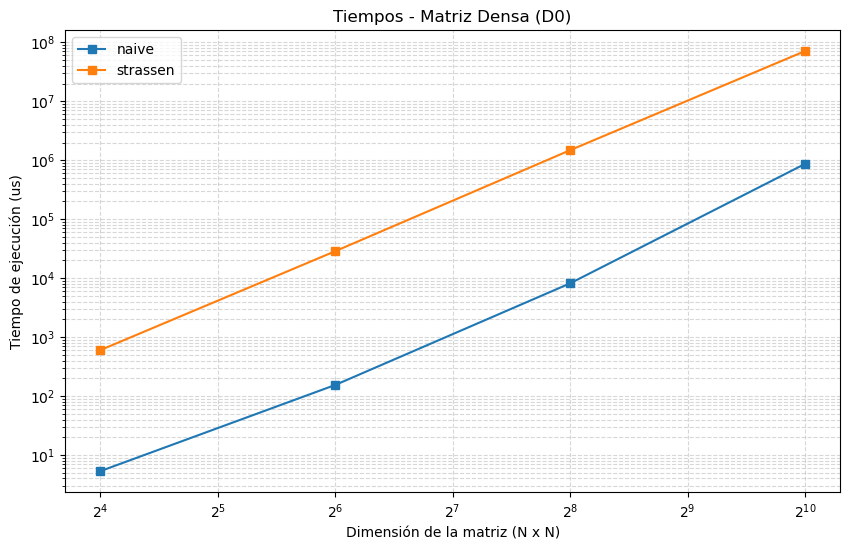
\includegraphics[width=0.7\linewidth]{sections/tiempos_densa_D0.png}
    \caption{Tiempo de ejecución en matrices densas (Dominio D0).}
    \label{fig:matrix_tiempo}
\end{figure}

A pesar de que en el papel Strassen ($N^{2.81}$) debería ganarle a Naive ($N^3$), en la práctica resultó sistemáticamente más lento en todas nuestras pruebas, sin importar el tipo de matriz ni el dominio. Esto se explica por dos grandes factores:
\begin{enumerate}
    \item El trabajo extra: aunque Strassen se ahorra 1 multiplicación (hace 7 en vez de 8), realiza cerca de 18 sumas y restas de matrices enteras en cada paso recursivo, lo cual es muy pesado y hace que se demore, en tiempo, más que Naive en casos grandes. 
    \begin{figure}[H]
        \centering
        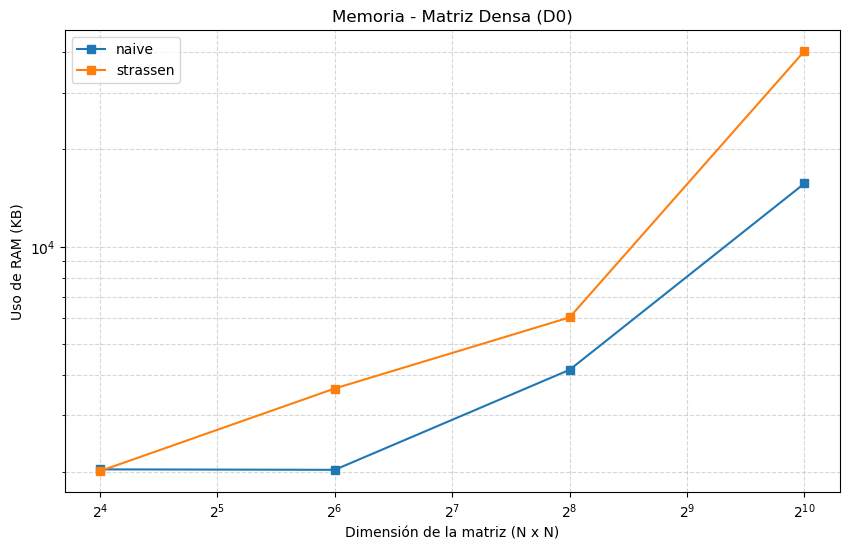
\includegraphics[width=0.7\linewidth]{sections/memoria_densa_D0.png}
        \caption{Consumo de memoria en matrices densas (Dominio D0).}
        \label{fig:matrix_mem}
    \end{figure}
    \item El problema de cómo está programado: ambos algoritmos representan las matrices como \verb|vector<vector<int>>| (un vector bidimensional). Esta forma de guardar datos hace que las filas queden dispersas en la memoria, provocando que al procesador le cueste más encontrarlas (mala localidad de caché). El detalle es que Naive reserva su memoria una sola vez al principio, mientras que Strassen, al ser recursivo, crea y destruye decenas de matrices pequeñitas temporales en cada uno de sus niveles. Esto multiplica la cantidad de veces que el sistema operativo debe asignar memoria, disparando tanto el tiempo real de ejecución como el consumo de RAM.
\end{enumerate}
En resumen, para que el algoritmo de Strassen empiece a ser más rápido que Naive en la vida real, se necesitan matrices muchísimo más gigantes que las de este laboratorio, además de programarlo usando arreglos planos.



